\chapter{The first chapter}

This chapter explains how to insert text correctly. Examples of the use of images, tables, listings, mathematical formulas and lists are also shown.



Let's start with the text. You start a new paragraph by leaving a blank line in the tex file. It does not matter how many blank lines there are in between.
However, line breaks without a blank line make no difference and are treated as a space character. To explain the spaces: The compiler never inserts more than one      space        between words.


You can write \textit{italic} by using the command \texttt{\textbackslash{}textit\{\}}, \textbf{bold} by using the command \texttt{\textbackslash{}textbf\{\}} and \underline{underlined} with \texttt{\textbackslash{}underline\{\}}. Words can be set in \enquote{quotation marks} by using \texttt{\textbackslash{}enquote\{\}}. Of course, those commands can all be \textit{\textbf{\underline{\enquote{combined}}}}. Besides that you can write \texttt{monospaced} with the command \texttt{\textbackslash{}texttt\{\}} which can be particularly useful for explaining commands or listings.

\subsubsection{Notice:}
The style of the quotation marks \enquote{...} is defined by the language. To change to English style, please edit \texttt{\textbackslash{}documentLanguage\{\}} in /content/settings.tex.

\section{First Section}
Subchapters are shown here.

\section{Second Section}
Text

\subsection{First Subsection}
Text

\subsection{Second Subsection}
Text

\subsubsection{First Sub-Subsection}
Text

\subsubsection{Second Sub-Subsection}
Text


\section{Figures}
An example figure is shown below.

\begin{figure}[H]
    \centering
    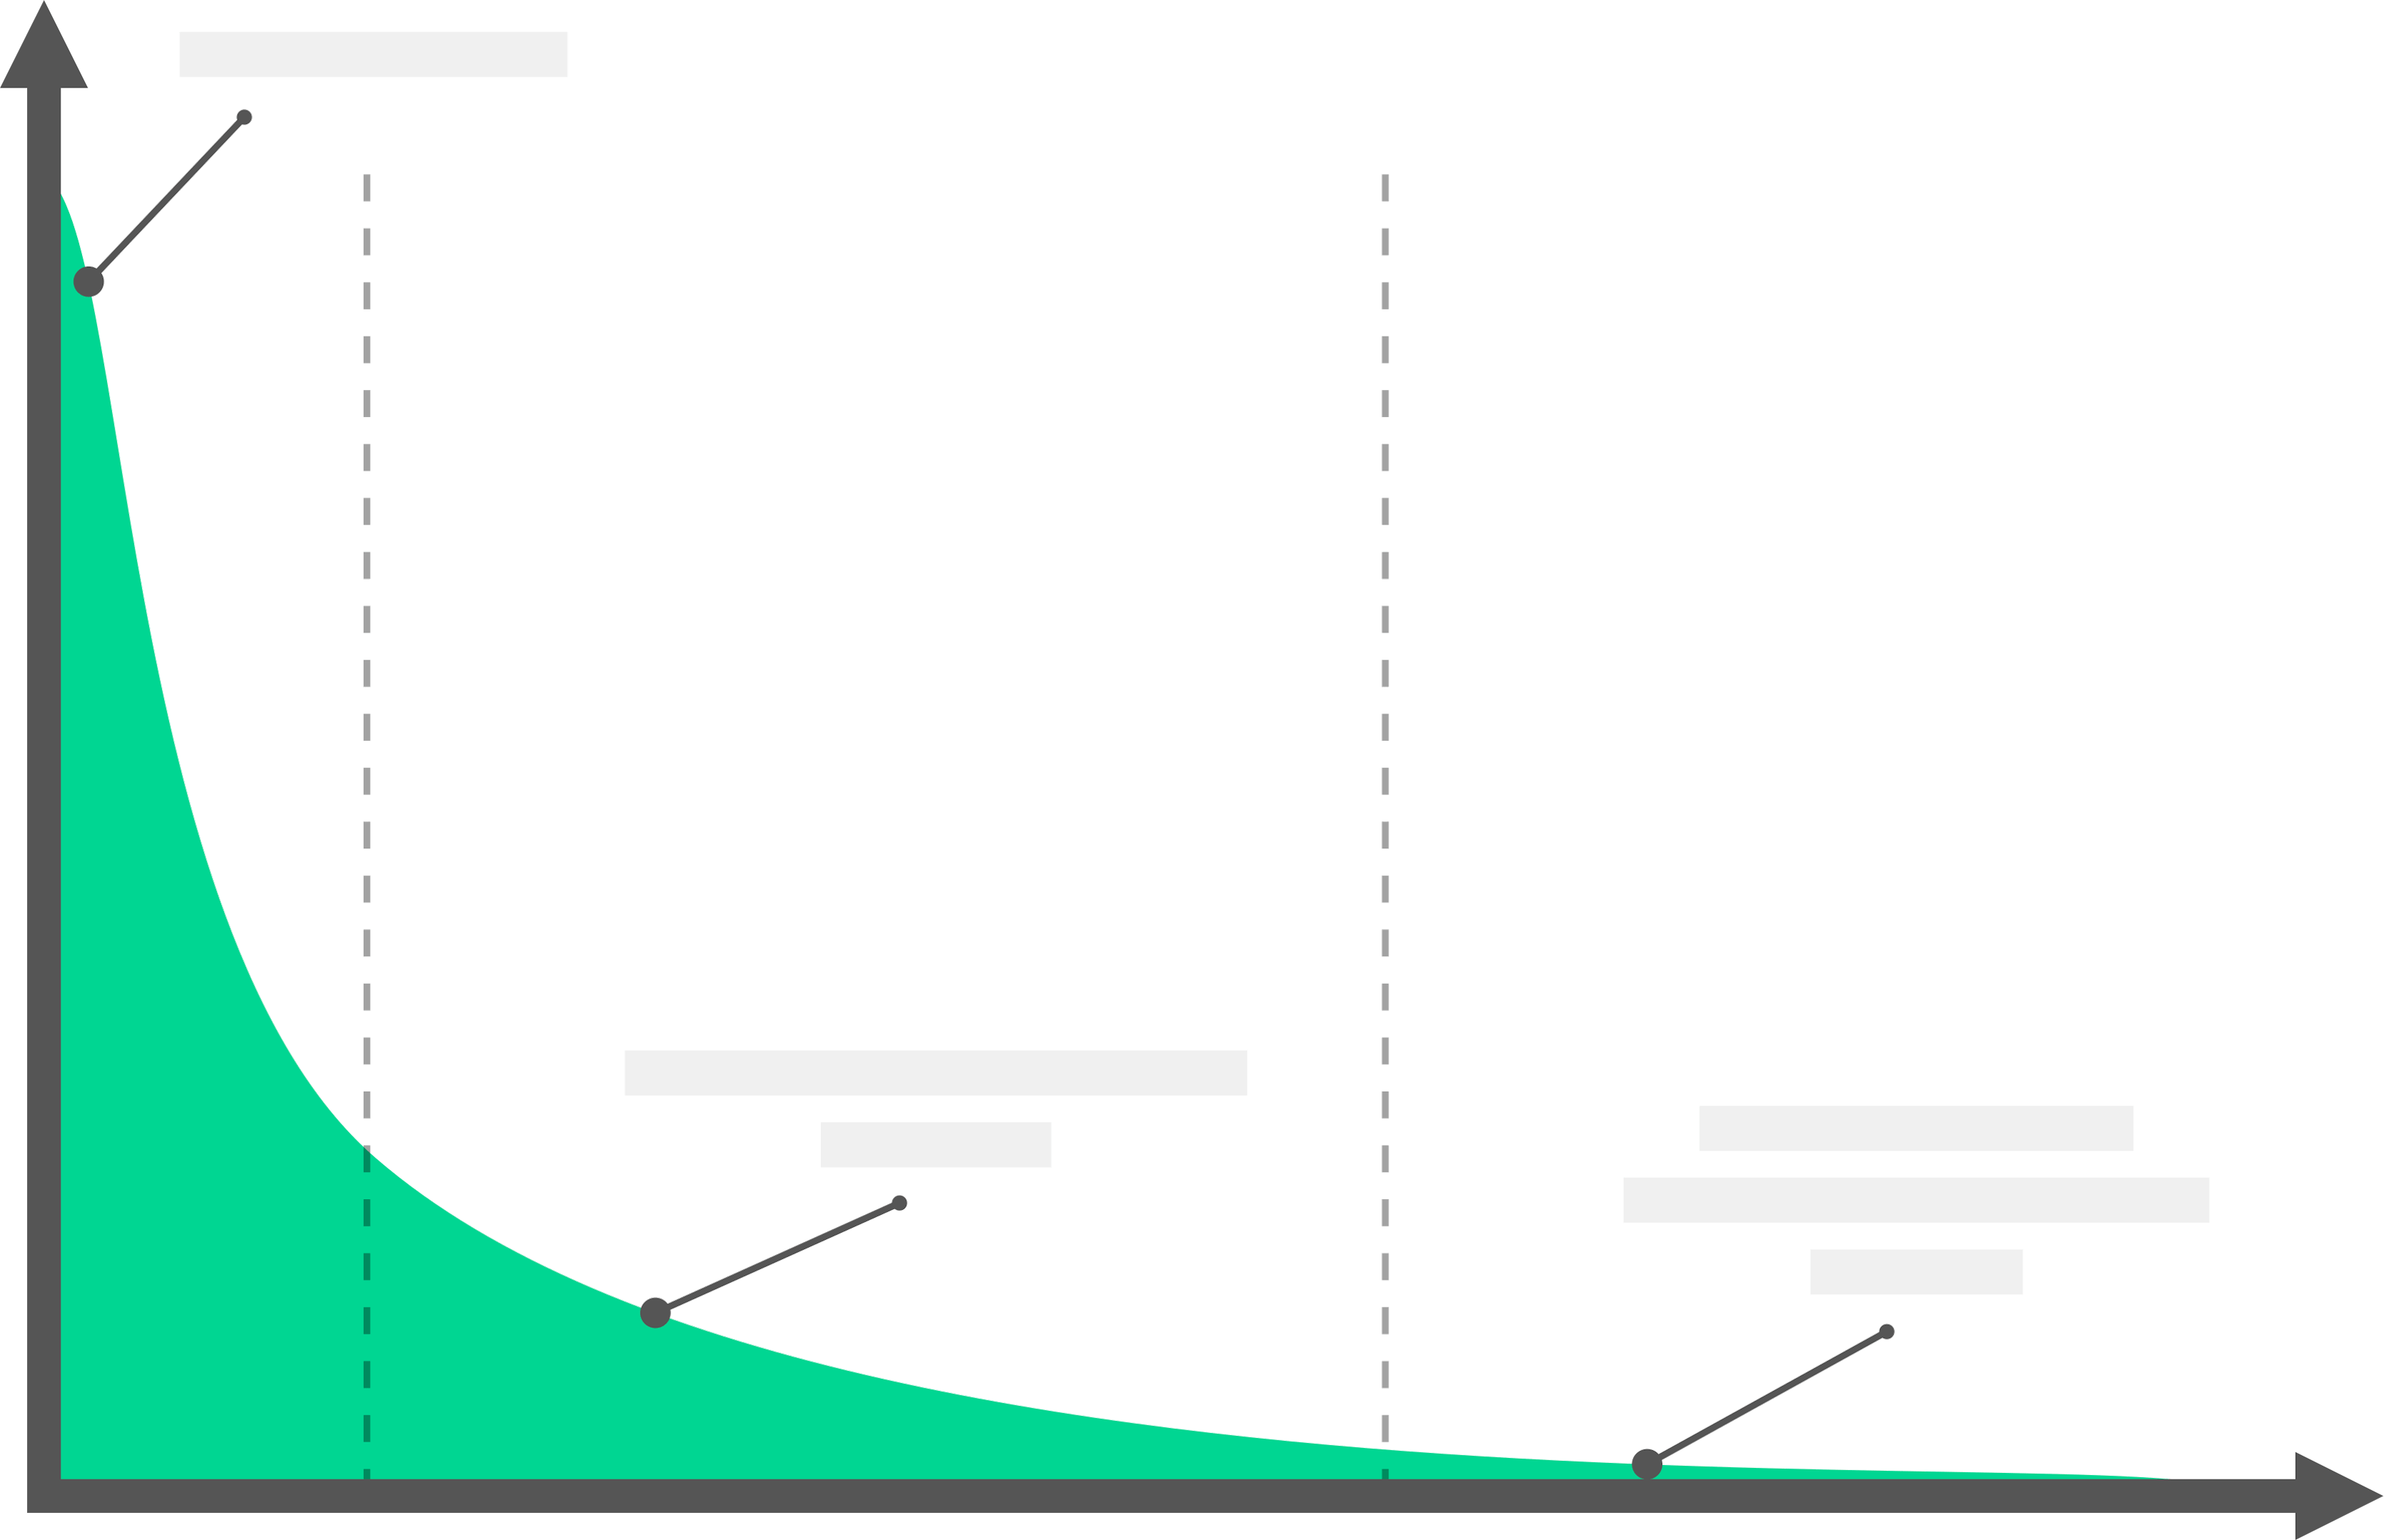
\includegraphics[width=0.7\linewidth]{FigureExample.png}
    \caption{My example figure}
    \label{fig:example}
\end{figure}

The image to be called up should be uploaded to the /content/images folder. The width of the image can be set with the \texttt{width} parameter. In this case, the image takes up 70\% of the text width (i.e. \texttt{width=0.7\textbackslash{}textwidth}). The 0.7 can take on values between 0 and 1, whereby the image then takes up the entire text width with the value 1.

It is recommended to copy exactly this code in order to insert other figures in the same way. However, the command \texttt{\textbackslash{}label\{\}} is only necessary if you want to refer to the image again later in the text.

The label can be named freely, but must not be defined the same way more than once. As can be seen in figure \ref{fig:example}, referencing images is very simple. All you need is the \texttt{\textbackslash{}ref\{\}} command.

\subsubsection{Pro-Tip:}
It is recommended to use vector graphics if possible. These usually require less storage space and have a much higher resolution than other pixel based formats. To use SVG, the command \texttt{\textbackslash{}includesvg[]\{\}} must be used.



\section{Tables}

The insertion of a table is explained here.

\begin{table}[H]
    \centering
    \caption{My example table}
    \label{tab:example}
    \begin{tabular}{|c|c|}
        \hline
        Cell A1 & Cell A2 \\
        \hline
        Cell B1 & Cell B2 \\
        \hline
    \end{tabular}
\end{table}

It is important here that the caption must always be above the table in accordance with the corporate design. The actual table (between \texttt{\textbackslash{}begin\{tabular\}} and \texttt{\textbackslash{}end\{tabular\}}) takes a little getting used to and is not necessarily self-explanatory to edit. For this reason, there are various tools on the internet that can help you to create a correctly formatted table in LaTeX. For example, \href{https://www.tablesgenerator.com/}{https://www.tablesgenerator.com/} or \href{https://www.latex-tables.com/}{https://www.latex-tables.com/}.

It is recommended to copy exactly this code in order to insert other tables in the same way. However, the command \texttt{\textbackslash{}label\{\}} is only necessary if you want to refer to the table again later in the text.

The label may be named freely, but may not be defined the same way more than once. As can be seen in table \ref{tab:example}, referencing tables is very simple. All you need is the \texttt{\textbackslash{}ref\{\}} command.


\section{Mathematical formulas}
Mathematical formulas are inserted as follows.

\begin{equation}
t-t_{0}=\sqrt{\frac{l}{g}}\int_{0}^{\varphi}{\frac{d\psi}{\sqrt{1-k^{2}\sin^{2} {\psi}}}} = \sqrt{\frac{l}{g}} F(k,\varphi)
\label{eq:example}
\end{equation}
\eqcaption{Example Caption in List of Equations}

The command \texttt{\textbackslash{}label\{\}} is only necessary if you want to refer to the formula again later in the text.

The label may be named freely, but may not be defined the same way more than once. As can be seen in the formula \ref{eq:example}, referencing formulas is very simple. All you need is \texttt{\textbackslash{}ref\{\}}.

There are various tools on the Internet that help to convert a formula or equation to LaTeX. Here is an example: \href{https://latex.codecogs.com/eqneditor/editor.php}{https://latex.codecogs.com/eqneditor/editor.php}


\section{Listings}
With listings, you can include essential parts of your program code.

\begin{lstlisting}[caption=My listing example, label=lst:example, language=C++]
public class HelloWorld {
	public static void main (String[] args) {
		// Output: Hello World!
		System.out.println("Hello World!");
	}
}
\end{lstlisting}

The listing formats the code directly in the correct language-specific colors. Spaces in strings are also highlighted. The parameter \texttt{language=...} needs to be adjusted for this to work correctly.

It is recommended to copy exactly this code in order to insert other tables in the same way. However, the command \texttt{label=...} is only necessary if you want to refer to the listing again later in the text.

The label can be named freely, but must not be defined the same way more than once. As can be seen in listing \ref{lst:example}, referencing listings is very simple. All you need is the \texttt{\textbackslash{}ref\{\}} command.


\section{Lists}
Sometimes you also need a list to list enumerations. This is created as follows.

\begin{itemize}
\item The first point.
\item The second point.
\item The third point.
\end{itemize}

This also works with numbers:

\begin{enumerate}
\item The first point.
\item The second point.
\item The third point.
\end{enumerate}